\documentclass[10pt,letterpaper]{article}

\usepackage[font=footnotesize]{caption}
\usepackage{float}
\usepackage{epsf}
\usepackage{epsfig}
\usepackage{subfigure}
% \usepackage{subfig}
\usepackage{latexsym}
\usepackage{color, colortbl}
\usepackage{wrapfig}
\usepackage{multirow}
\usepackage{tabularx}
\usepackage{hyperref}
\usepackage{xcolor}
\usepackage{mdwlist}
\usepackage{pdfpages} 

%\usepackage{color}
\newcommand{\lc}[1]{\textcolor{blue}{#1}}


\usepackage{amsmath, amsfonts, amssymb}
\usepackage[hmargin=1in,vmargin=1.2in]{geometry}
\usepackage{url}
\usepackage{multirow}
\usepackage[ruled,noline,linesnumbered]{algorithm2e}
\usepackage[bottom]{footmisc}
\usepackage{afterpage}
%\usepackage[caption=false]{caption}
\usepackage{eurosym}
\usepackage{enumitem}
% \usepackage{soul}
\usepackage{fancyhdr}
\usepackage{dashrule}
% \usepackage[stable]{footmisc}
% \usepackage{placeins}
% \setitemize{noitemsep,topsep=0pt,parsep=0pt,partopsep=0pt}
% \usepackage[utf8]{inputenc}
% \usepackage{gensymb}
% \usepackage{rotating}
% \usepackage{tikz}
% \usepackage[firstpage]{draftwatermark} 

% \SetWatermarkText{DRAFT}
% \SetWatermarkScale{1}
% \SetWatermarkLightness{0}

% \interfootnotelinepenalty=80 
% \floatingpenalty=0\relax
\widowpenalty=1000
\clubpenalty=1000

\def\ls{{\texttt{LSTS\ }}}
\def\lse{{\texttt{LSTS}}}
\def\nas{{\texttt{NASA\ }}}
\def\nase{{\texttt{NASA}}}
\def\onr{{\texttt{ONR\ }}}
\def\onre{{\texttt{ONR}}}
\def\noa{{\texttt{NOAA\ }}}
\def\noae{{\texttt{NOAA}}}
\def\onrg{{\texttt{ONR Global\ }}}
\def\onrge{{\texttt{ONR Global}}}
\def\dar{{\texttt{DARPA\ }}}
\def\dare{{\texttt{DARPA}}}
\def\auk{{\texttt{AUKUS\ }}}
\def\auke{{\texttt{AUKUS}}}


\def\org{{\texttt{RAND\ }}}
\def\orge{{\texttt{RAND}}}
\def\dec{{\texttt{UN Decade of the Oceans\ }}}
\def\dece{{\texttt{UN Decade of the Oceans}}}


\interfootnotelinepenalty=10000

\def\etal{{et al.\/}}
\def\eg{e.g., }
\def\ie{{i.e.,\ }}
\def\etc{{etc.\ }}
\def\situ{{in situ \/}}
\def\PN{{\emph{PN} }}


\input{epsf}

%\usepackage{mathptmx}
%\usepackage{multirow}

\newcommand{\rtime}[1]{\par\noindent\rlap{#1} \hspace*{2.15cm}}
\newcommand{\iblank}{\par \noindent \hspace*{2.4cm} \hangindent 2.6cm}
\newcommand{\m}[1]{\ensuremath{\mathbf{#1}}}
\newcommand{\mc}[1]{\ensuremath{\mathcal{#1}}}
% \newcommand{\mb}[1]{\mbox{\boldmath$#1$\unboldmath}}
%\newcommand{\norm}[1]{\left| \left| #1 \right| \right| ^2}
\newcommand{\snr}{\hbox{SNR}}
\newcommand{\mse}{\hbox{MSE}}
\newcommand{\E}{{\mathbb E}}
\newcommand{\cn}{{\mathcal{CN}}}
\newcommand{\ba}{\begin{align*}}
\newcommand{\ea}{\end{align*}}

\newcommand{\real}{{\mathbb{R}}}
\newcommand{\integer}{{\mathbb{Z}}}
\renewcommand{\natural}{{\mathbb{N}}}
\newcommand{\argmin}{\operatorname{argmin}\displaylimits}
\newcommand{\argmax}{\operatorname{argmax}\displaylimits}

\newcommand{\relthresh}{{T_{\text{rel}}}}
\newcommand{\absthresh}{{T_{\text{abs}}}}

\newcommand{\nprof}{{N_{\text{prof}}}}
\newcommand{\DM}{{DM}}
\newcommand{\UM}{{UM}}
\newcommand{\deltaMax}{{\partial_{\max}}}
\newcommand{\IFD}{{IFD}}
\newcommand{\IFU}{{IFU}}

\newcommand{\mvdiff}{\mathbf{mvd}}
\newcommand{\mvest}{\widehat{\mvdiff}}
\newcommand{\prof}{p}

\newtheorem{Prop}{Proposition}
\newtheorem{Theorem}{Theorem}
\newtheorem{Lemma}{Lemma}
\newtheorem{Corrolary}{Corollary}

\def\be{\begin{equation}}
\def\ee{\end{equation}}

\newlength{\doublespacelength}
\setlength{\doublespacelength}{\baselineskip}
\addtolength{\doublespacelength}{0.5\baselineskip}
\newcommand{\doublespace}{\setlength{\baselineskip}{\doublespacelength}}

\newlength{\singlespacelength}
\setlength{\singlespacelength}{\baselineskip}
\newcommand{\singlespace}{\setlength{\baselineskip}{\singlespacelength}}


\newlength{\savedspacing}
\newcommand{\savespacing}{\setlength{\savedspacing}{\baselineskip}}
\newcommand{\restorespacing}{\setlength{\baselineskip}{\savedspacing}}

\setlength{\parskip}{0pt}
\setlength{\parsep}{0pt}
\setlength{\headsep}{0pt}
\setlength{\topskip}{0pt}
\setlength{\topmargin}{0pt}
\setlength{\topsep}{0pt}
\setlength{\partopsep}{0pt}
% \setlength{\parindent}{0pt}

\newtheorem{definition}{Definition}
\newcommand{\icomnt}[1]{{\color{red}{#1}}}
\newcommand{\kcomnt}[1]{{\color{blue}{#1}}}
\newcommand{\unit}[1]{\ensuremath{\mathrm{#1}}}                  %%%% to units and other roman math stuff
% \linespread{0.98}
% % \linespread{2.00}

\newcommand{\siftaddress}{319 1st Ave. N., Suite 400\\
Minneapolis, MN~~~55401}

\newcounter{quotenumber}

\newenvironment{numquote}{%
    \begin{enumerate}%
     \setcounter{enumi}{\value{quotenumber}}%
     \color{darkgray}
    \item \begin{quote}%
}{%
    \end{quote}%
    \setcounter{quotenumber}{\value{enumi}}
    \end{enumerate}%
}%

\makeatletter
\def\myitem{%
   \@ifnextchar[ \@myitem{\@noitemargtrue\@myitem[\@itemlabel]}}
\def\@myitem[#1]{\item[#1]\mbox{}}
\makeatother



\newcommand\blankpage{%
    \null
    \thispagestyle{empty}%
    \addtocounter{page}{-1}%
    \newpage}

\setcounter{secnumdepth}{0} 

\let\oldthebibliography\thebibliography
\let\endoldthebibliography\endthebibliography
\renewenvironment{thebibliography}[1]{
  \begin{oldthebibliography}{#1}
    \setlength{\itemsep}{0em}
    \setlength{\parskip}{0em}
}
{
  \end{oldthebibliography}
}
% \linespread{0.98}
\parskip 0.1cm
\definecolor{Gray}{gray}{0.6}

\title{Memo: An \auke-wide initiative on Autonomous Systems}
\author{% \textsf{\large{Kanna Rajan}}\\
  % \emph{Kanna.Rajan@rand.org}\\
  % \url{https://kanna.rajan.systems
  }
\begin{document}

\maketitle{}

\subsection{Background}

\begin{wrapfigure}{!h}{3.5in}
  \centering
  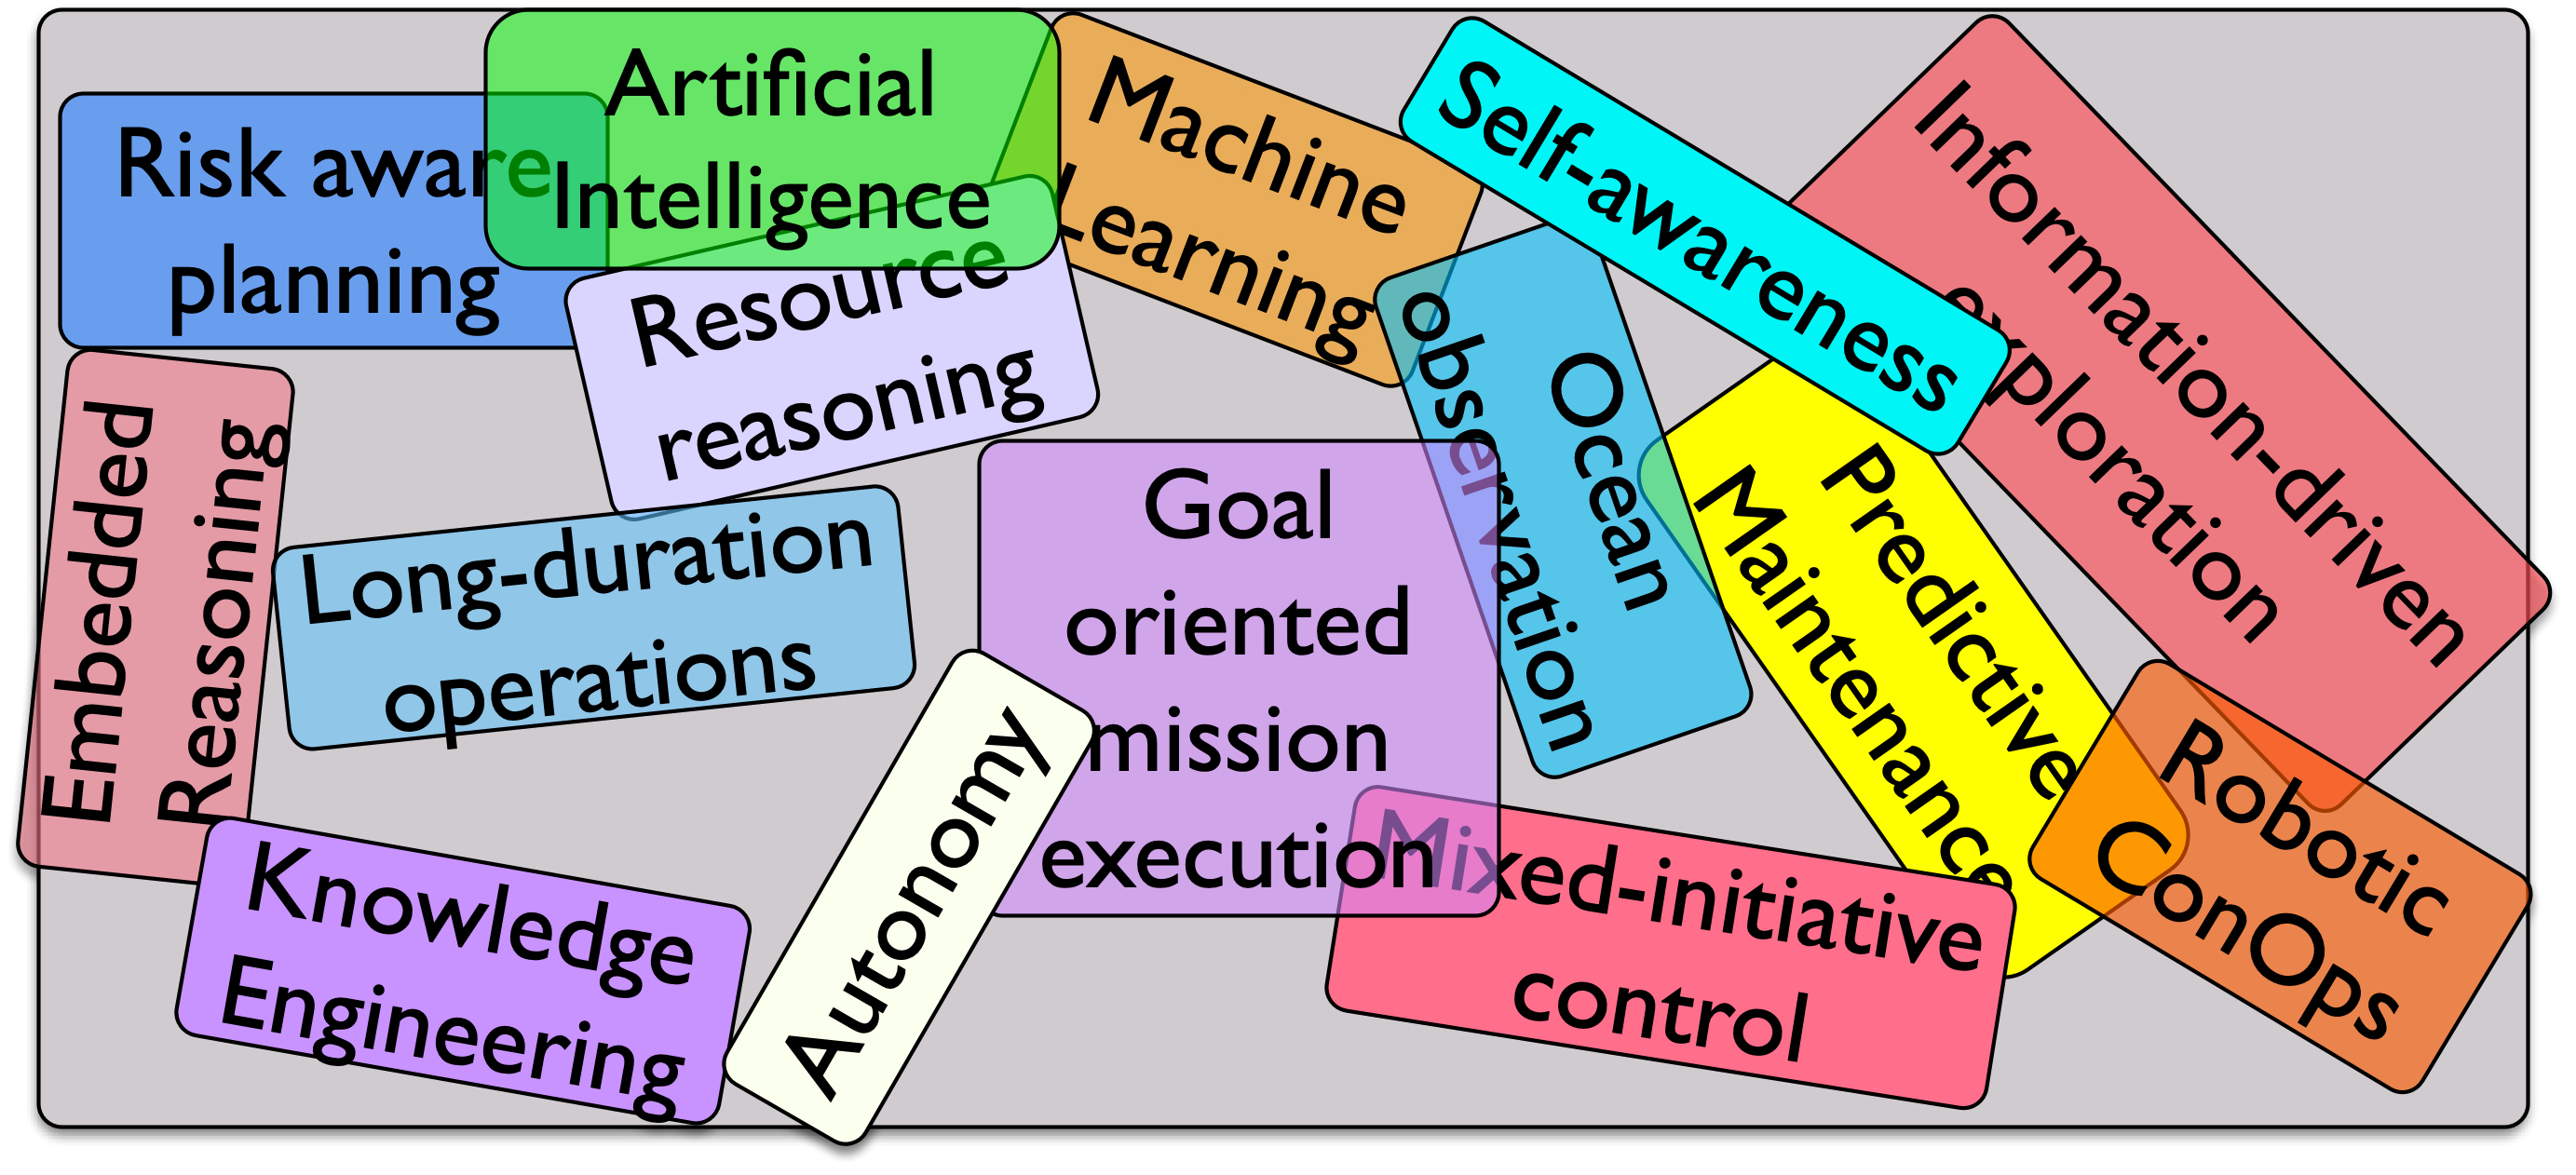
\includegraphics[scale=0.09]{fig/word-bag.jpg}
  \caption{}
 \label{fig:topics}
\end{wrapfigure}

Autonomous unmanned systems have made steady progress in their
capabilities driven in large part by the ubiquity and scaling effect
of sensors and computational platforms. Starting as niche experimental
platforms confined to structured laboratory environments, they have
not only been in used in space, but increasingly in operational
real-world environments relevant to militaries the world over
demonstrated as never before in the Ukraine conflict. Such systems are
being introduced across multiple domains (Fig. \ref{fig:systems})
across aerial, on land and water, as well as underwater. To these we
include the increasingly contested space domain, where low-cost (in
the millions of \$'s) small satellites are playing significant roles
in remote sensing and intelligence gathering. Autonomous platforms
have been operating in multiple aerial domains across the world for
sometime; they are increasingly operating in the Persian Gulf, the
Black Sea, the Carribean and the South China Sea to name a few. Land
based systems such as the Robotic Combat Vehicle are planned to be
inducted; \noae's use of manned airplanes going thru Category 4 \& 5
hurricanes for data collection have given way to the successful use of
unmanned surface vehicles. 

The primary \emph{modus-operandi} of such systems for now has been via
mixed-initiative (i.e. human-in-the-loop) control. This has allowed
placing the human well outside harms way, while also providing an
extension of the human senses. The technology roadmap of such systems
however, calls for 'dialing up' the autonomy in ways that embedded
machine intelligence (at the core of AI) can make decisions, drive
towards goal achievment and recover from failures, enabling robustness
and consistency in mission operations. Whether they augment the
warfighter, or completely replace them is likely to depend on a range
of issues spanning technology readiness to policy implications of such
self-aware fighting machines.

While \org efforts have touched on such system capabilities, the
policy implications related to their resurgance and the implication of
fighting wars and in-turn how such capabilities could impact a range
of issues including foreign policy, defense aquisition,
recruitment/retention all the way to mission capabilities, operations
and posture, have not been adequately studied. We believe it is time
to do so. 
 
\begin{figure}[h!]
\centering
\vspace{-0.3in}
\subfigure[]{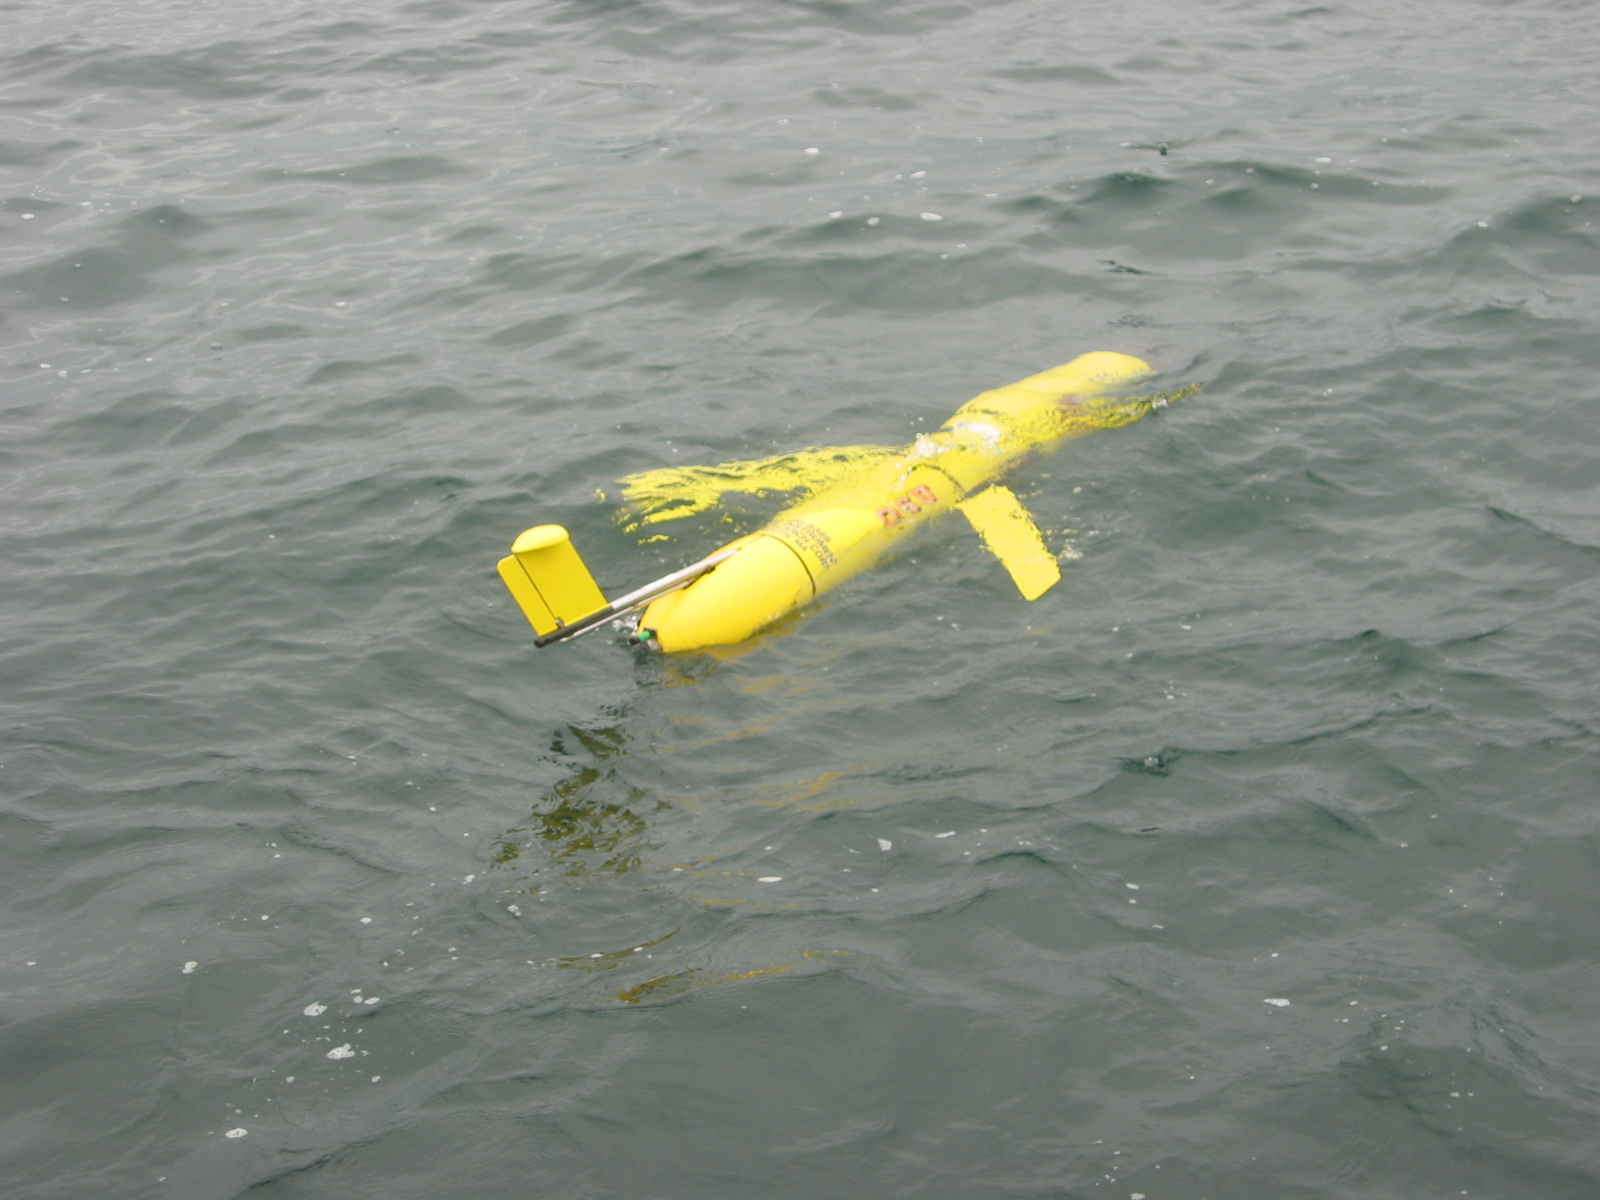
\includegraphics[height=1.68in]{fig/glider.jpg}\label{fig:auv}}
\subfigure[]{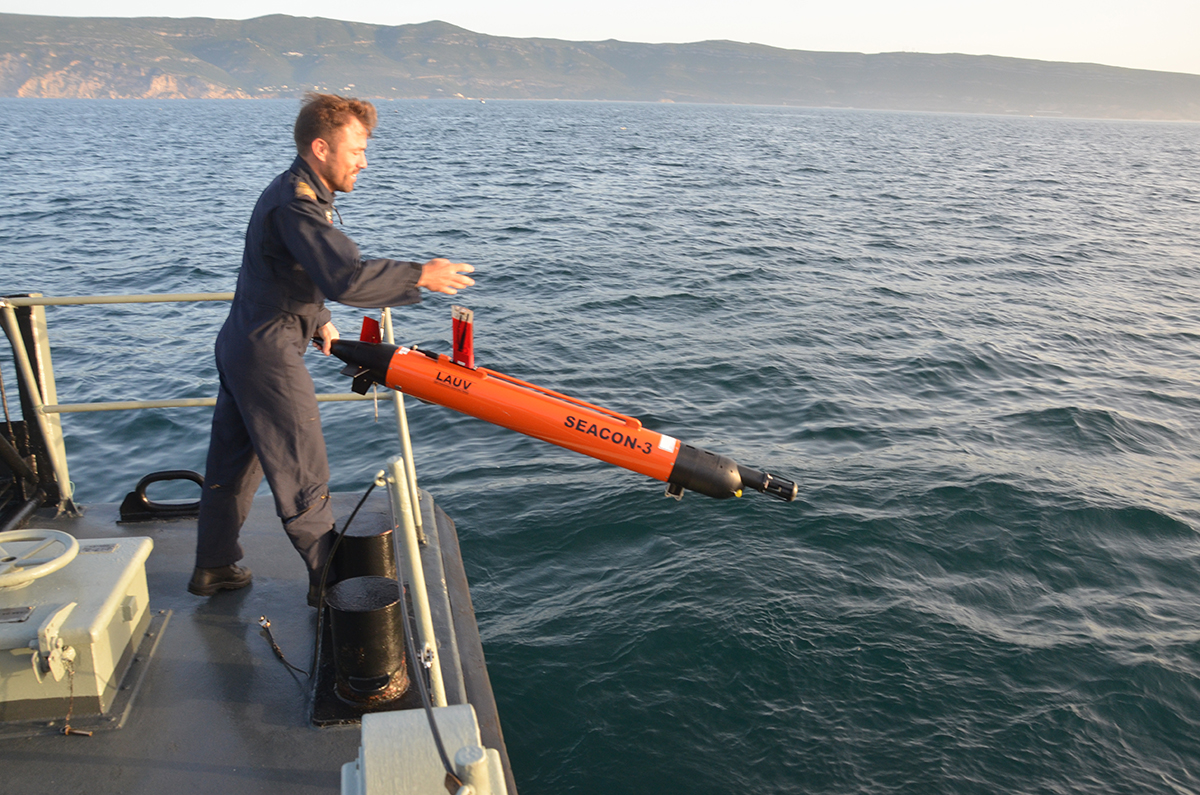
\includegraphics[height=1.68in]{fig/DSC_9044.jpeg}\label{fig:lauv}}
\subfigure[]{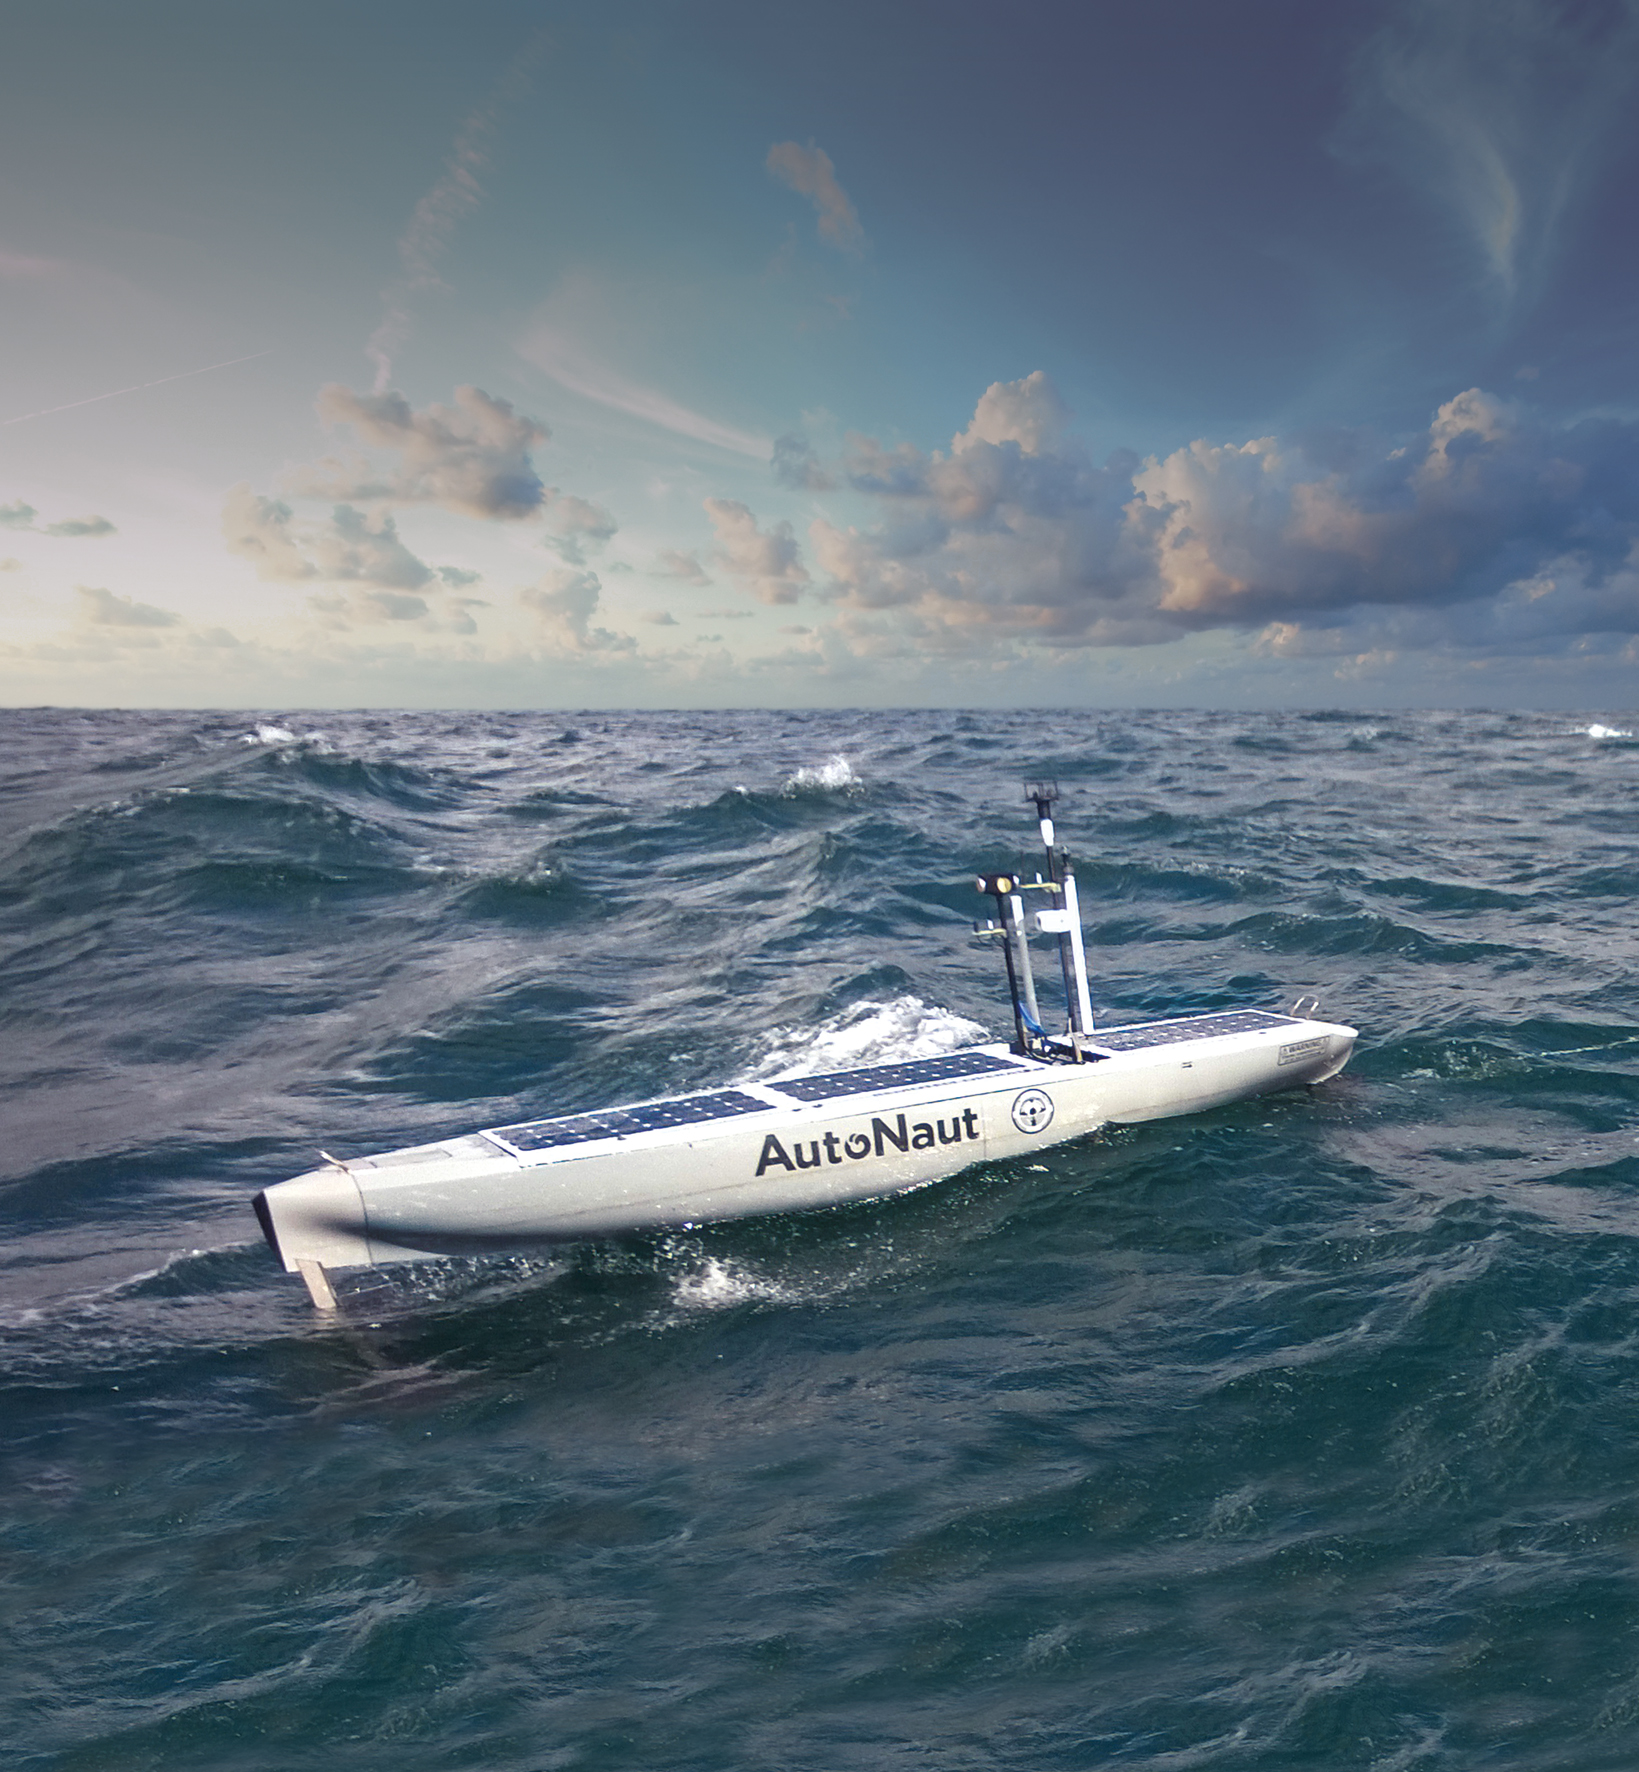
\includegraphics[height=1.68in]{fig/AutoNaut4.jpg}\label{fig:asv}}
\subfigure[]{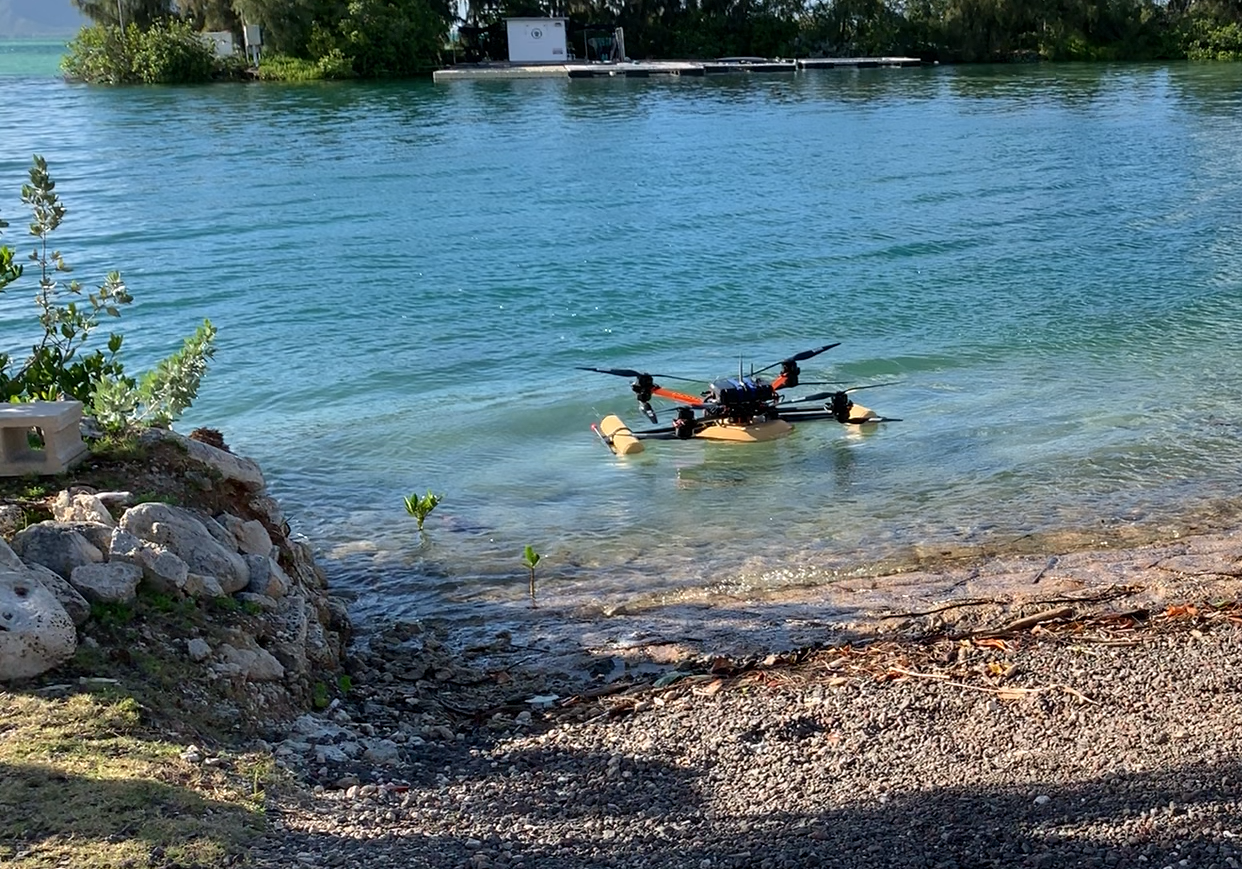
\includegraphics[height=1.68in]{fig/titan_in_water.png}\label{fig:uav}}
\caption{ \subref{fig:auv} Glider - an unpropelled Autonomous
  Underwater Vehicle.  \subref{fig:lauv} A propelled Autonomous
  Underwater Vehicle (AUV), deployable from shore or ship.
  \subref{fig:asv} An Autonaut wave-energy driven autonomous surface
  vehicle (ASV).  
  \subref{fig:uav} An Unmanned Aerial Vehicle (UAV) dual-quadcopter.}
\label{fig:systems}
\end{figure}


\subsection{Proposal}

We propose to establish an \auke-wide Unmanned System initiative
within \org to position it as a thought leader in the policy,
regulatory and ethical dimensions of the use of unmanned systems in
military and quasi-military (e.g. Coast Guard) environments. By doing
so, \org will tap into its \emph{existing} expertise in shaping how
agencies in the US, UK, the EU and Australia are working
collaboratively from the conceptual use to actual operations of
unmanned systems across space, aerial, surface (terrestrial and
oceanic), underwater and underground domains.

There are three key reasons for such an initiative to span \auke-wide.
One is \orge's own visible footprint in these geographical
entities. Another and equally important reason is the increasing
coordination and collaboration between the entities in \auke. Finally,
the technology induction process across \auk is likely to be similar
given its levels of acceptance and maturity across these
regions. Finally, by joining forces across these nations, \org can
rapidly and efficiently help augment the existing collaborations and
connections in the various forces and agencies and be in a position to
rapidly provide 'lessons learned'.

As a result, the focus of such an initiative will be on shaping
policies that foster the use and application of autonomous unmanned
systems while ensuring safety, security, and societal acceptance
across a large geographical and political swath.


\subsection{Path forward at \org}

We propose the following implementation plan:

\begin{description}

\item[Establish a core team]: Form a multidisciplinary team of \org
  experts in robotics, AI, sensors, acquisition and operations

\item[Funding and Partnerships]: Secure funding through existing or
  new government grants (i.e. NSRD), private foundations, and industry
  sponsorships subject to review

\item[Project Pipeline]: Identify and initiate high-impact policy
  research projects, prioritizing those with potential to influence
  regulatory frameworks and societal norms
  
\item[Outreach and engagement]: Promote the portfolio’s activities
  through conferences, OpEds, commentaries and media outreach


\end{description}

\subsubsection{Ambition}

Our longer term objective would be a single 'go to' entity within \org
which will span across various divisions, including DPS, SEW, NDRI,
HSRD and the FFRDC's. This entity could be a 'center' which can then
be used as a focal point not just for cross-cutting work in autonomous
systems, but also for chanelling funding including from philanthropies
and non-DoD sponsors, such as \noae, Schmidt Ocean Institute, \ldots.


\end{document}